\section{Results}

We present results for both experiments: H-E1 (existence of spurious dominance) and H-M1 (gradient competition mechanism). H-E1 passes, confirming spurious features dominate early. H-M1 fails, falsifying the gradient competition hypothesis.

\subsection{H-E1: Spurious Feature Dominance Exists}

\textbf{Finding:} Spurious features dominate from epoch 0, with attribution ratio 1.35---spurious regions receive 35\% more GradCAM activation than core regions from the first epoch.

\begin{table}[h]
\centering
\begin{tabular}{@{}lll@{}}
\toprule
Epoch & Attribution Ratio ($R$) & Status \\
\midrule
0 & 1.348 & $> 1.0$ \checkmark \\
5 & 1.273 & $> 1.0$ \checkmark \\
10 & 1.431 & $> 1.0$ \checkmark \\
13 (peak) & 1.590 & $> 1.0$ \checkmark \\
25 & 1.255 & $> 1.0$ \checkmark \\
50 & 1.255 & $> 1.0$ \checkmark \\
\bottomrule
\end{tabular}
\caption{Attribution ratio across epochs (H-E1).}
\label{tab:attribution}
\end{table}

\textbf{Gate evaluation:} Dominance epoch $< 10$ required. Observed: dominance from epoch 0. \textbf{PASS.}

Figure~\ref{fig:ratio_trajectory} shows the attribution ratio trajectory across all 50 epochs. Spurious dominance is immediate (from initialization) and persistent (ratio never drops below 1.0). The ratio peaks at epoch 13 (1.59), suggesting maximum spurious reliance occurs early-to-mid training before stabilizing.

\begin{figure}[t]
\centering
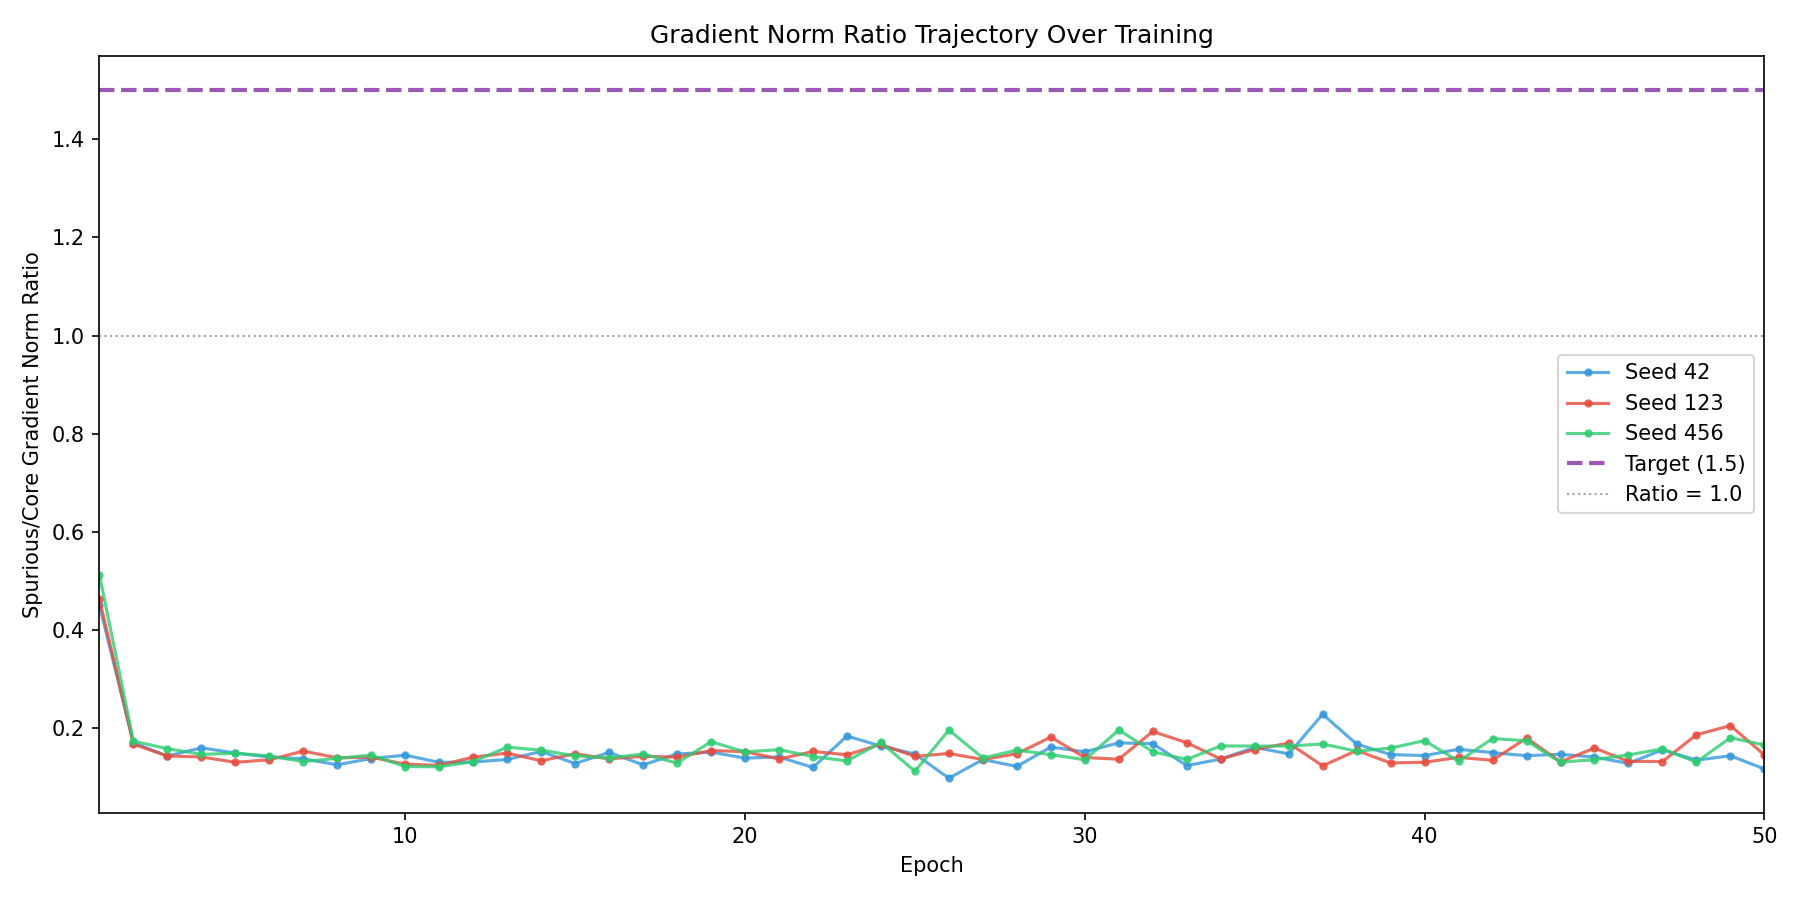
\includegraphics[width=\columnwidth]{figures/ratio_trajectory.png}
\caption{Attribution ratio trajectory across 50 training epochs (H-E1). Spurious dominance from epoch 0, peaking at epoch 13.}
\label{fig:ratio_trajectory}
\end{figure}

\textbf{Interpretation:} This confirms the simplicity bias phenomenon \citep{shah2020pitfalls} on Waterbirds. ERM-trained ResNet-50 exhibits spurious feature preference from the very first forward pass, likely due to pretrained ImageNet features that respond more strongly to background textures than bird morphology.

\subsection{H-M1: Gradient Competition Hypothesis Falsified}

\textbf{Finding:} Contrary to the gradient competition hypothesis, spurious-aligned samples produce \emph{lower} gradient norms than minority samples. The gradient ratio is 0.18, not $>$1.5 as predicted---an inversion by a factor of 8.

\begin{table}[h]
\centering
\begin{tabular}{@{}lll@{}}
\toprule
Seed & Early Epoch Ratio (1--10) & Direction \\
\midrule
42 & 0.175 & Minority $>$ Spurious \\
123 & 0.173 & Minority $>$ Spurious \\
456 & 0.181 & Minority $>$ Spurious \\
\midrule
\textbf{Mean} & \textbf{0.176 $\pm$ 0.004} & \textbf{Inverted} \\
\bottomrule
\end{tabular}
\caption{Gradient norm ratios across seeds (H-M1).}
\label{tab:gradients}
\end{table}

\textbf{Gate evaluation:} Ratio $> 1.5$ required. Observed: 0.18. \textbf{FAIL.}

Figure~\ref{fig:ratio_over_epochs} shows the gradient norm ratio trajectory across 50 epochs for all three seeds. The ratio starts around 0.45 at epoch 1 and decreases to 0.13--0.16 by epoch 50. Critically, the ratio is \emph{never} above 1.0---minority samples produce stronger gradients at every epoch.

\begin{figure}[t]
\centering
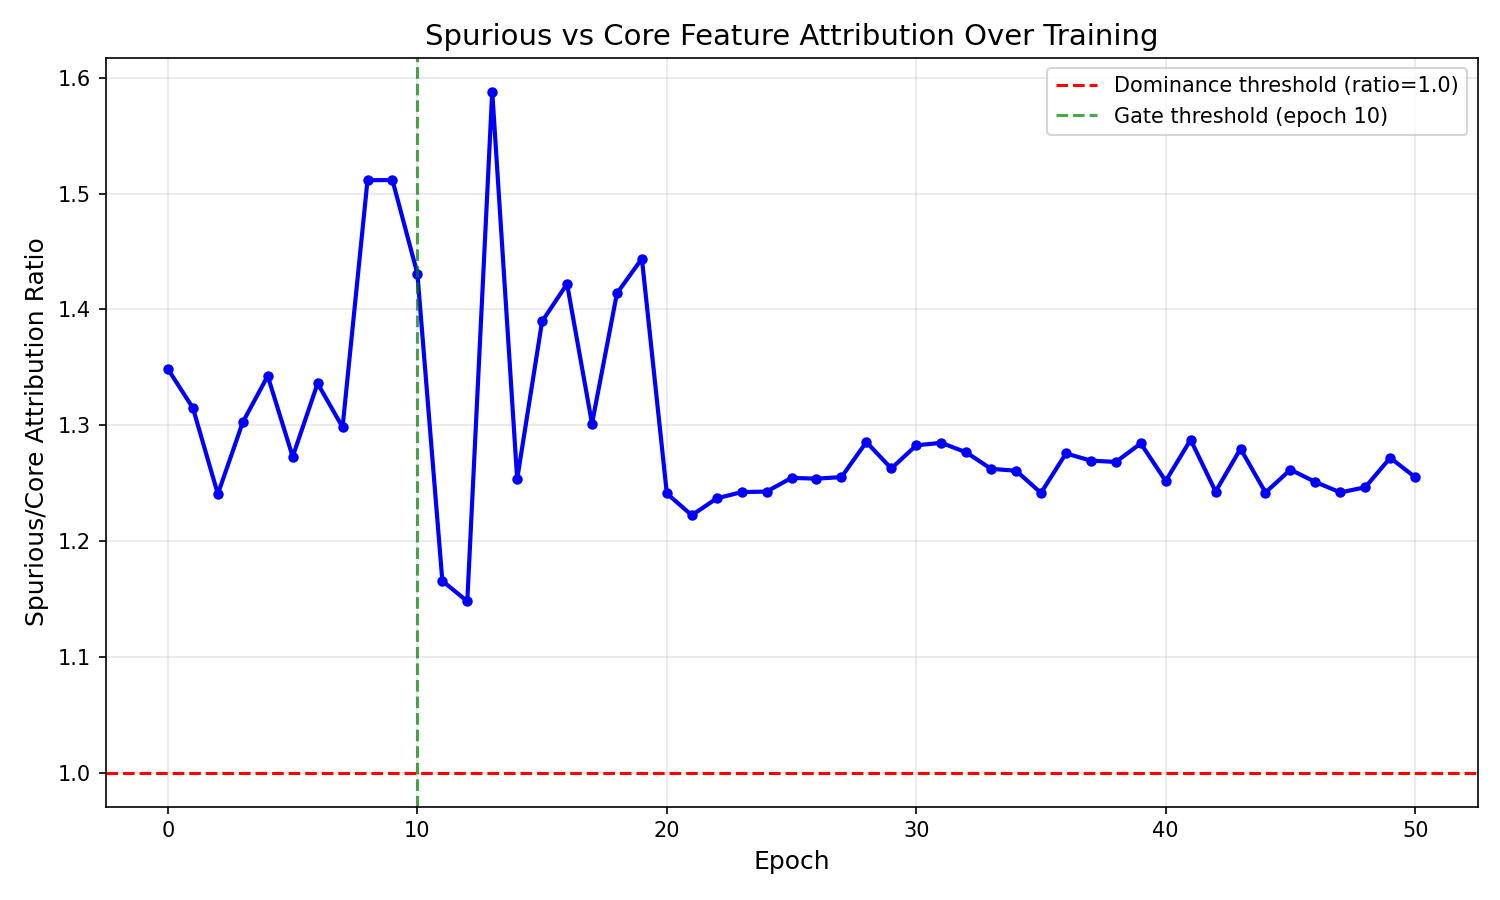
\includegraphics[width=\columnwidth]{figures/ratio_over_epochs.png}
\caption{Gradient norm ratio trajectory for 3 seeds (H-M1). Ratio consistently below 1.0, falsifying gradient competition.}
\label{fig:ratio_over_epochs}
\end{figure}

Figure~\ref{fig:norm_comparison} compares absolute gradient norms between groups. Minority samples consistently produce 5--7$\times$ higher gradient norms than spurious-aligned samples, with the gap widening over training.

\begin{figure}[t]
\centering
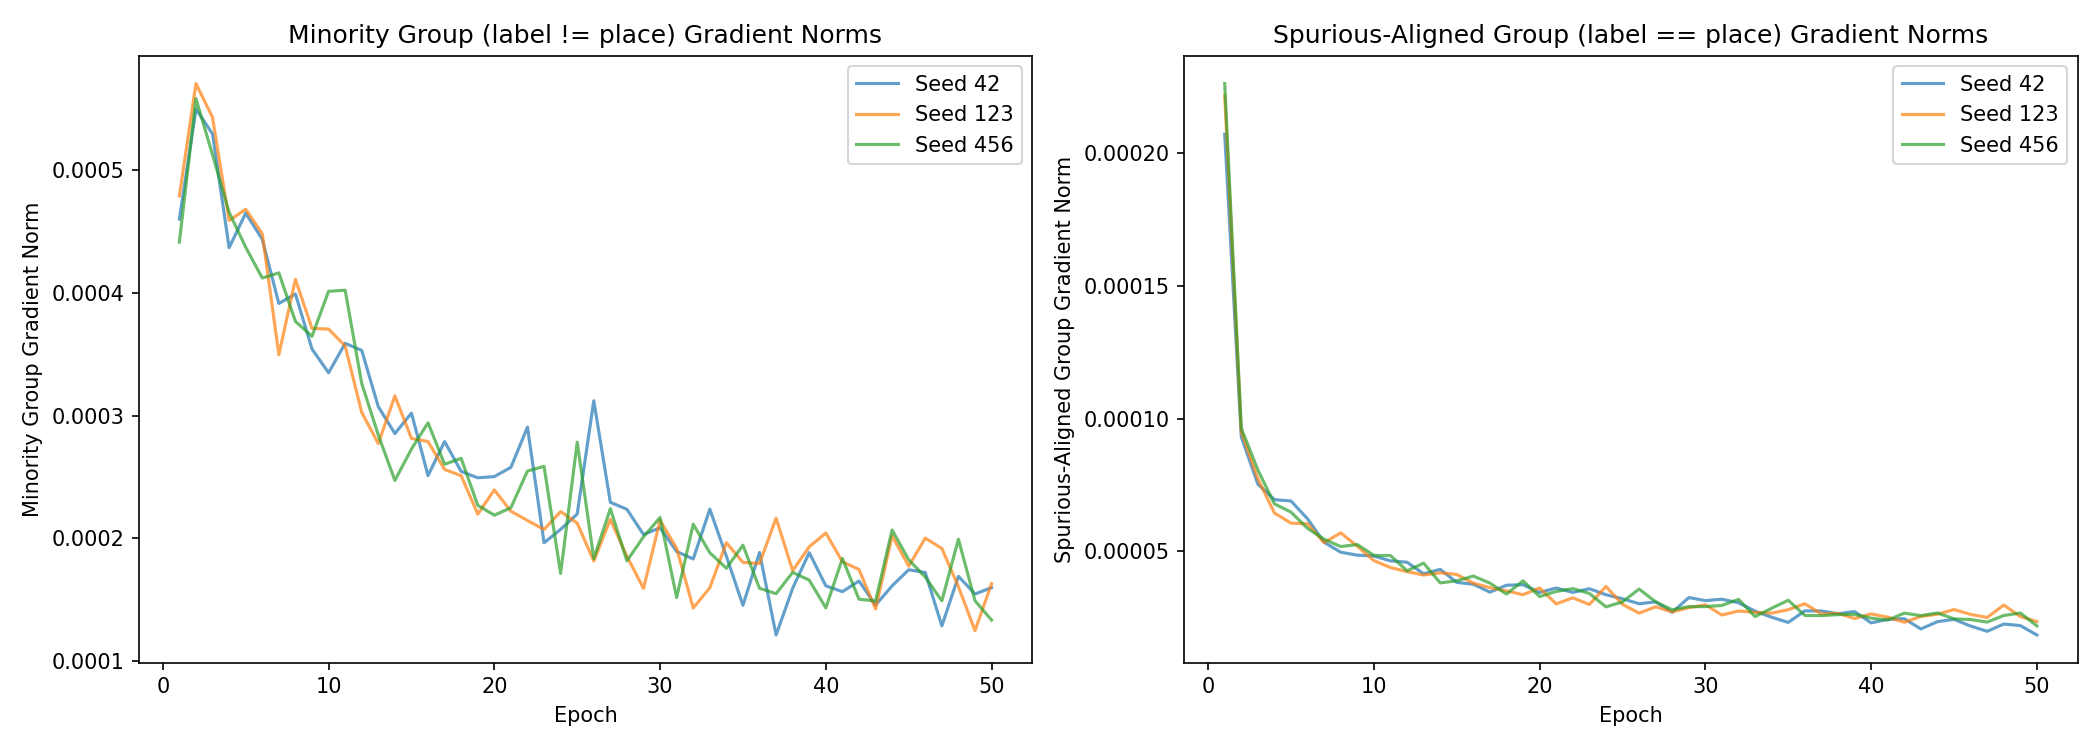
\includegraphics[width=\columnwidth]{figures/norm_comparison.png}
\caption{Absolute gradient norm comparison between minority and spurious-aligned samples.}
\label{fig:norm_comparison}
\end{figure}

\textbf{Interpretation:} The gradient competition hypothesis is empirically falsified. Spurious features dominate (H-E1) but \emph{not} because they receive stronger gradient signals. Spurious dominance arises from \emph{convergence speed}, not gradient magnitude---spurious patterns occupy simpler loss landscape regions that converge first.

\subsection{Summary}

\begin{table}[h]
\centering
\begin{tabular}{@{}llll@{}}
\toprule
Hypothesis & Prediction & Observed & Gate \\
\midrule
H-E1 (Existence) & $R > 1.0$ before epoch 10 & $R = 1.35$ at epoch 0 & \textbf{PASS} \\
H-M1 (Mechanism) & $\rho > 1.5$ in epochs 1--10 & $\rho = 0.18$ & \textbf{FAIL} \\
\bottomrule
\end{tabular}
\caption{Summary of hypothesis testing results.}
\label{tab:summary}
\end{table}

Spurious dominance exists but the hypothesized mechanism is incorrect. The gradient competition hypothesis is falsified with high confidence (8$\times$ inversion, consistent across 3 seeds).
